% Created 2019-04-16 Tue 14:23
% Intended LaTeX compiler: pdflatex
\documentclass[12pt,a4paper,man]{report}
\usepackage[utf8]{inputenc}
\usepackage[T1]{fontenc}
\usepackage{graphicx}
\usepackage{grffile}
\usepackage{longtable}
\usepackage{wrapfig}
\usepackage{rotating}
\usepackage[normalem]{ulem}
\usepackage{amsmath}
\usepackage{textcomp}
\usepackage{amssymb}
\usepackage{capt-of}
\usepackage{hyperref}
\renewcommand{\baselinestretch}{1.5}
\usepackage{apacite} \usepackage{algorithm} \usepackage{listings} \usepackage[noend]{algpseudocode}  \usepackage{indentfirst}  \usepackage{fancyhdr} \usepackage{stringstrings}
\usepackage[table]{xcolor}
\usepackage{longtable}
\usepackage{geometry} \geometry{ a4paper,  total={170mm,257mm}, left=20mm, top=1in, foot=0.3in}
\usepackage[final]{pdfpages}
\usepackage{placeins}
\usepackage{cmap} \usepackage[T1]{fontenc}
\usepackage[raggedright]{titlesec}
\usepackage[toc,section=section]{glossaries}
\makeglossaries
\usepackage{minted} %minted requires -shell-escape flag. Remove it if necessary
\author{Ibrahim M. Shaatha, Faith Alfred}
\date{\today}
\title{Final Report I: Affective Movie Evaluator}
\hypersetup{
 pdfauthor={Ibrahim M. Shaatha, Faith Alfred},
 pdftitle={Final Report I: Affective Movie Evaluator},
 pdfkeywords={},
 pdfsubject={},
 pdfcreator={Emacs 26.1 (Org mode 9.1.9)}, 
 pdflang={English}}
\begin{document}

%enable heading 4
\setcounter{secnumdepth}{4}
\titleformat{\paragraph}
{\normalfont\normalsize\bfseries}{\theparagraph}{1em}{}
\titlespacing*{\paragraph}
{0pt}{3.25ex plus 1ex minus .2ex}{1.5ex plus .2ex}

\newglossaryentry{FER}{
         name={FER},
         description={Facial Expression Recognition.}
}

%set the first page
\setboolean{@twoside}{false}
\begin{titlepage}

\includepdf[pages=-,pagecommand={},width=\textwidth]{FirstPage.pdf}
\end{titlepage}
\maketitle
\tableofcontents
\listoftables
\listoffigures

%FIX ISSUE WITH CHAPTER TITLE MARGIN
\makeatletter
\@addtoreset{chapter}{part}
\def\ttl@mkchap@i#1#2#3#4#5#6#7{%
  \ttl@assign\@tempskipa#3\relax\beforetitleunit
  %\vspace*{\@tempskipa}% NEW
  \global\@afterindenttrue
  \ifcase#5 \global\@afterindentfalse\fi
  \ttl@assign\@tempskipb#4\relax\aftertitleunit
  \ttl@topmode{\@tempskipb}{%
    \ttl@select{#6}{#1}{#2}{#7}}%
  \ttl@finmarks  % Outside the box!
  \@ifundefined{ttlp@#6}{}{\ttlp@write{#6}}}
\makeatother 

%CHAPTER TITLE STYLE
\titleformat{\chapter}[hang] 
  {\normalfont\huge\bfseries}
  {\chaptertitlename{ \thechapter : } }
 {0in}
  {} 


\newpage
\begin{abstract}
  For our final year project we are building an application that analyses videos of audience watching movie and gives the video a score called  the Affective Movie Evaluator. We established the goals and objectives and we were able to achieve roughly half of our objectives. This report is a summary of the conception, developement and of the project. We also discuss the current progress of the project and future plans briefly. 
\end{abstract}

\newpage
\topskip0pt
\vspace*{\fill}
\section*{Declarations}
I hereby declare that the report presented here as part of the requirement of BIT304 is original and no parts of this report had been plagiarised from any other resources unless those indicated with proper referencing.  This report will be the property of HELP University and cannot be distributed in any form without the written consent of HELP University.
\\\\Student Names:
\begin{description}
 \item Mohamed Shaatha Ibrahim (B1301746)
 \item Elebe Faith Alfred (B1301511)
\end{description}
Date: 12-04-2019
\vspace*{\fill}

\renewcommand{\abstractname}{Acknowledgement}
\begin{abstract}
	Aknowledgements
	This project will not be possible without the help of a number of people. We would like to express our deepest gratitude to HELP's University Department of Information and Communication Technology for their support and provision to make this project a success and to our family for their unconditional love and support to make sure our education is successful.

Our gratitude goes to the following individuals who have been with us through this journey:
Ms. Shu Mn for teaching and guiding us through the entire process of this project
Mr. Abdul Quayoon for being patient with us as our supervisor, and for providing insight and expertise that has greatly helped us in implementing our project

And we also thank our Colleagues who have been of help to us in the best way that they can.
\end{abstract}



%set the header
\newcommand\SentenceCase[1]{
  \caselower[e]{#1}
  \capitalize[q]{\thestring}
}
\newcommand*\parttitle{}
\let\origpart\part
\renewcommand*{\part}[2][]{%
   \ifx\\#1\\% optional argument not present?
      \origpart{#2}%
      \renewcommand*\parttitle{#2}%
   \else
      \origpart[#1]{#2}%
      \renewcommand*\parttitle{#1}%
   \fi
}

\pagestyle{fancy}
\fancyhf{}
\rhead{\thepage}
\lhead{\parttitle{}: \leftmark}
\cfoot{\thepage}
\renewcommand{\chaptermark}[1]{\markboth{#1}{}}

\part{Proposal}
\label{sec:org4bdb545}
\chapter{Introduction}
\label{sec:org516f2bb}

Movie production studios use test screening in order to determine whether their movies will succeed. Recently, internet movie distributors such as Netflix and Amazon have started taking more control of the production of their content, it is more beneficial for studios to re-edit their movie once they can predict that the product is going to fail. While there are automated sentiment analysis tools used to measure how well the audience reacts to test screening, most of the feedback is still taken from questionnaires and the audiences subjective evaluation.

We aim to provide an automated, movie evaluation system which is going to analyse the audience watching the movie and predict an overall score. Our system is intended to supplement the existing manual process of test screenings. We are not proposing a system to replace the existing subjective evaluations given by the audience.

The aim of this project is to develop a system that can evaluate how good a movie is, by analysing both face and body postures of the audience. In order for this to work we provide the system a video file consisting of audience reactions, and the system will tell us how good a movie is within a rating metrics, we will define later. It is important for us to state, that we are not proposing a real-time system here; the system accepts a recording of the raw data - which is currently defined as video file, and can be any other form of measurement - as the primary input.

A system like this can aid us develop further, a more general system that can evaluate how good a certain product or presentation is by analysing the audience reaction limited by a certain context. In our case the product is a movie, and how the audience reacts may depend on what genre of movie they are watching, or what kind of experience they were expecting beforehand. It is likely that our system may not work well without knowing these information. Systems like these are also related to computer vision with Emotion AI technologies, such as face based lie detectors, which uses the same techniques to work.

\chapter{Background}
\label{sec:org84b1a24}
For a long time movie industry have used statistical modeling and machine learning to predict, the success of movies based on high level data. While there have been several works in early to mid 2000’s, which takes in multimedia information to form a representation for the user’s emotions \cite{Shiliang_Zhang_2008,wu2008interactive}, the earliest work we could find that specifically focus on movie scenes was by Soleyman et. al.

Quite recently, there have been interest in using deep learning techniques to analyse audiences facial data such as \cite{saha2018unsupervised}, to predict whether an audience enjoyed the movie, most notably research work that has been funded by The Walt Disney Company \cite{Deng_2017}. The purpose of their research is to use facial emotion recognition techniques, to analyse the emotion of the audience in order to improve the movies.

Research has shown that over 90\% of our communication can be non – verbal (Algorithmia, 2018). Non- verbal communication which includes facial expressions and body postures among others can be used to determine the emotional state of a human being. According to Paul Ekman (Ekman P, 1992), there are basically six types of human emotions namely:  happiness, sadness, disgust, fear, surprise, and anger. 

The system we are proposing is going to take in a video file of an audience reacting to a movie and attempts to determine whether the audience liked that movie. It will use emotion recognition and body pose to quantify the overall reaction in order to determine whether the viewer enjoyed the movie or not. 

Although, idea of such a system is not new, we have not been able to find an existing system that considers both body pose and facial emotion data to create a model that can predict. Previous work such as (V Ramanarayanan et al., 2015), which evaluates a presenter by using a very similar technique that we are planning, performed very poorly compared to the human judges. However, we are a bit more optimistic, since movies are designed to elicit certain emotional responses and audiences in average exhibit similar reactions. Such a system, maybe useful in the film industry to analyse the reactions of the test audience as a supplement to the usual questionnaires. 
The problem we are trying to solve is that film studios screens movies to test audience, and audience writes back a subjective feedback usually on paper. Our software is intended to complement the existing evaluation procedure, by providing an automated evaluation of audience's experience that is less subjective and provide a numerical score that represents audience's sentiment more accurately.

Affective Analysis is already used by marketing giants such as Coca-Cola to predict the effectiveness of their advertisement on target test audiences. Affective movie analysis could prove to be valuable to streaming services that distributes their own content and have more control over the productions such as NetFlix.

\chapter{Issues}
\label{sec:org60a0100}
Our system is not real-time but still requires heavy computing power in order to run. This means the admin will often have to run multiple processes for analysis and come back later for the result. Our system does not support multiple processes yet, while it is possible for our system to run a process on a remote server or a cloud computer service via ssh and http, the admin still have to wait for the analysis to be completed. 

In order to minimize the scale of the problem, the first few iterations of the problem deals with only a single audience member. The largest audience we will be designing our system will be for a group of two to four person, under controlled lighting environment. Unless we have access to infrared cameras and better computing facilites, we will not be able to overcome these limitations. 

Our video can only have one person in front of the camera. The application is not able to give proper result if there are faces in the background when the audience member is reacting. Presence of another person in the room currently effects the resulting data, and it is very time consuming for a human to verify whether the recorded data does not have any background face. However, as we wrote our detection algorithm to choose the largest region of interest in the image, the fail cases we have observed usually consists of background posters and wallpapers with larger face than our subject.

One of the weakness we have is in the accuracy of the face detection algorithm. OpenCV's default facial detection algorithm, (Viola-Jones full frontal model) requires the audience member to face the camera directly. However, we plan to implement a more accurate face detection algorithm at the risk of increasing computing time.

Right now our system uses an externel media player known as VLC media player, to play the movie while being recorded in use case 1. The system admin is usually required to install the software manually. However on Windows based systems, it is sometimes not possible to find the 

\chapter{Benefits and Constraints}
\label{sec:orgf4439d8}
For our current iteration the system can analyse only one audience member. The reason for this limitation is that we initially wanted to start the project with a smaller scope and also to reduce the amount of tasks we might have for the first iteration. Even in our future iterations, we will not be analysing and audience consisting of more than a handful of person, unless we get better camera equipments.

Another issue faced by us is that facial emotion recogntion is not working that well, for now. In order to improve the accuracy of the \gls{FER} model we plan to write separate test cases.

Since our system takes a long time to analyse, we had to modify our "Analyse Video" use case into two seperate parts. Instead of directly providing a video file to run analysis and immediately getting the results and visualisations, our system actually requires the admin to run two seperate instance of analysis, facial emotion analysis (FER) and pose analysis (BEGR). Running an instance of analysis will produce the required data file, which can then be visualised as a time-series and processed to be sent for our movie evaluation ML model.


\chapter{Project Aims and Objectives}
\label{sec:org399c5f7}
The aim of our project is to develop a system that can evaluate how good a movie is, by analysing both face and body postures of the audience. In order for this to work we provide the system a video file consisting of audience reactions, and the system will tell us how good a movie is within a rating metrics, we will define later. It is important for us to state, that we are not proposing a real-time system here; the system accepts a recording of the raw data - which is currently defined as video file, and can be any other form of measurement - as the primary input.
\begin{itemize}
\item system like this is very useful for movie studios, which often relies on test audience in order to predict whether their movies are going to be successful and a system like this can aid in measuring the audience reaction more accurately.
\end{itemize}
The objectives we have set for our project are the following:
Define the metrics by which the system is going to give the score before we create the evaluation model. (e.g: value between 0.0-1.0 or a discrete grading system, like A+, A,  
\begin{itemize}
\item Research the requirements of the dataset, and methodologies before week 3.
\item Find or create the required test datasets for in order to complete objective 6.
\begin{itemize}
\item Dataset for the emotion recognition subsystem
\item Dataset for body pose subsystem.
\item Dataset for the whole system: Video recordings of audiences reacting to movies.
\item Determine accuracy of the overall project by comparing its output to existing scoring systems.
\end{itemize}
\item To prove that we are using state of the art technologies in our system; produce:
\begin{itemize}
\item Accuracy report for Emotion recognition
\item Accuracy report Body pose/action estimation
\end{itemize}
\end{itemize}

\chapter{Project Scope}
\label{sec:orgd84ea22}
\begin{itemize}
\item For developement purpose, we will be dealing with short movies mostly.
\item We will be recording atleast 12 subjects, watching multiple movies.
\end{itemize}

Before we proceed, we would like to borrow a very recent terminology from Andrej Karpathy that has been in use in the industry. \emph{Software 2.0} refers to any software that is written without direct human involvement, with the help of another software. We chose to use this term in document to highlight the fact that the developement approach and the documentation practices used for the machine learning portions of the code is slightly different than the rest, and it will not be honest from our part to describe the process as the same. Though term originated in an article he wrote, we have seen the term used within a very few academic papers \cite{ratner2018snorkel}. In contrast, \emph{Software 1.0} refers to any type of software that a human is directly responsible for creating and we will be only using the term to distinguish it, if necessary.

A large portion of the project is in Software 2.0, therefore we do realize we have to spend a lot of time collecting data, analysing the data and evaluating our application. For this reason our primary methodology is described as SEMMA methodology, even though for iteration 1 we actually use a mixed method.


\chapter{Software and Hardware Requirements}
\label{sec:org0d3d41d}

\section{Funding Sources}
\label{sec:org68b147f}
As mentioned before we do not have any corporate and industry backing, therefore we are expecting HELP School of ICT to provide any possible funding we may require, if requested. Since the University already have most of the assets we require for our FYP1, we will require permission from the IT department to use the facilities, for our project.
As for FYP2, the tools and resources we require for data collection and obtaining ground truth can only be determined after we complete the first part of our project.

\section{Minimum hardware requirements}
\label{sec:org109ce80}
Although, our system can run with a laptop with a webcam we designed the system with the following requirements in mind.

\begin{table}[htbp]
\caption{\label{table:mreq}
Minimum Hardware Requirements}
\centering
\begin{tabular}{|l|l|l|l|lp{3cm}|}
\hline
No & Item & Usage & Qty\\
\hline
1 & VGA USB Camera & Used to record audience & 1\\
\hline
2 & Computer Terminal & Our application need to run & 1\\
 & (Desktop/Laptop & on an computer with a & \\
 & /SmallFactor) & display terminal. & \\
\hline
\end{tabular}
\end{table}

\section{Recommended hardware requirements}
\label{sec:org283ed4d}

\begin{table}[htbp]
\caption{\label{table:mxreq}
Recommended Hardware Requirements}
\centering
\begin{tabular}{|l|l|l|l|lp{3cm}|}
\hline
No & Item & Usage & Qty\\
\hline
1 & HD Camera & Used to record audience & 1\\
2 & High-end Desktop Computer & Our application need to run & 1\\
 &  & on an computer with a & \\
 &  & display terminal. & \\
3 & CUDA compatible Graphics & Used to improve video & 1\\
 & Card - NVDIA geforce & analysis models & \\
 & gtx 1080 ti &  & \\
\hline
\end{tabular}
\end{table}

\chapter{Development Methodology}
\label{sec:orgcbe3b29}
To give you the context of the reasoning behind our decision, we would like to discuss a brief overview of commonly used development methodologies first. The most commonly followed methodologies for data-science projects are either SEMMA or CRISP-DR methodologies. SEMMA is a methodology developed by SAS institute, while CRISPR-DR method was originally developed in a joint effort by five companies, and further improved by data mining industry, most notably by IBM. 

The main difference between both methodologies are that CRISPR-DR considers business understanding of the process and also considers model deployment and the results. SEMMA is mainly used for data mining projects, which does not consider business aspect. The methodology we chose for our project is SEMMA methodology.

The reason we chose SEMMA is that, we wanted to keep option generalise our problem scope later, for example we wanted to apply what the system does in other scenarios than movies. Also, business project timelines and research project timelines are usually incompatible, and this is a fact we need to consider while planning early on, since machine learning projects falls under the latter. So not considering the business aspects of the project, will be an advantage for us given the time we  have. 

\begin{figure}[htbp]
\centering
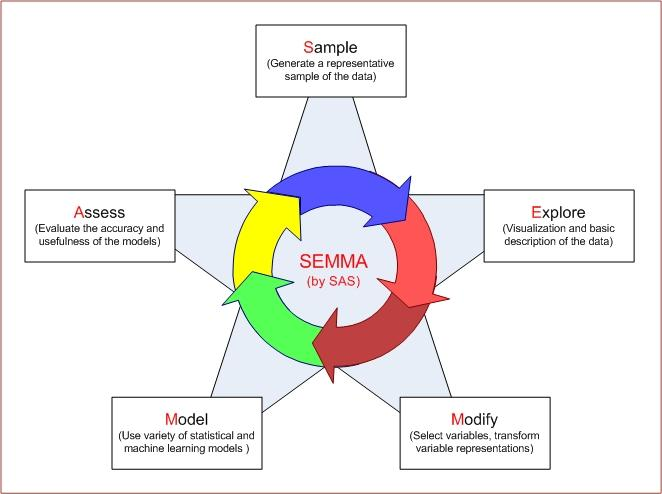
\includegraphics[width=6in]{./ext_img/SEMMA.JPG}
\caption{SEMMA (2018, Data Mining for Business Intelligence Series)}
\end{figure}

SEMMA methodology consists of 5 phases (Sample, Explore, Modify, Model and Assess). SEMMA methodology gives us freedom to reiterate from any step, as we require. It does not have a definitive cycle for iteration, which makes it a more simple and less rigid framework to follow, compared to CRISP-DR (Palacios, 2017). 
Sample:  First step of of SEMMA involves collecting all data samples.
Explore: Understand the problem through exploration of sample data. Exploration can be helped through visualisations and other data analytic tools.
Modify: Next steps, involves selecting which variables/features can be used, how they can be transformed or processed in order to create a model.
Model phase consists of selecting and creating a model
Assess: Finally we evaluate how well the model performed, and determine whether it is useful in real world situation.
In order to properly use SEMMA methodology into our project we are going to we are going to collectively apply the methodology to three separate components of our system that we have previously identified; the facial emotion subsystem, body emotion subsystem and movie evaluation model. After we started planning, we realized given only two team members, it was actually impossible for us to go through the whole system with one iteration within one semester. 

Therefore, we have split the project into two phases. Each phase is considered iteration by itself, because during the first phase, we build the first two components of our pipeline simultaneously (by two members), such that they both go through the SEMMA process at the same time. During the process, we also ensure both components are integrated before we start the next phase.

Then, we will start next iteration; go back to the sample stage to work on the final part of our project. For example, after the Assess phase of the emotion models we will be starting again from Sample phase again, and ensure everything in the pipeline is working well. This does not mean we define the term “phase”  and “iteration” as being interchangeable. 

Eventually, given the results it is possible we may plan a new iteration, if necessary. For example, if after assessing the Movie Evaluation Model, it performed poorly, we may go back to either Modify stage to pick better features to be passed into the model or we can even go back to Model stage to pick a different model.

The first planned iteration of  our project we will be focused on building the facial emotion and body pose emotion subsystem, which will be for simplicity hence referred to as “Emotion Model” and “Pose Model”, respectively. The second part of our project will be the combined system along with “Movie Evaluation Model”. Most of our work on Movie Evaluation Model, is currently planned to commence on the second part of our internship (FYP2), and the gantt chart we have proposed in the Appendix section might significantly change.

As our primary version control system we will be using gitlab as our github repository. Also, since SEMMA does not define a project management style, we will be using kanban/scrum like board feature on gitlab, to organize the tasks that we will be doing. However, we will not be adhering to any strict project management style, which is very prevalent in the software industry.

As for the specific techniques we will use throughout the development, our idea is to analyse existing literatures, and compare notes and follow general data mining/modeling techniques with fewer brainstorm sessions. In order to obtain the ground truth while collecting the data, our current idea is to use questionnaires after recording a subject’s reaction. Alternatively, it’s possible for us to measure blood pressure or any other means of observation if possible, and we will consider that for our FYP2.

\part{Project Management Plan}
\label{sec:org7bf7302}
\chapter{Introduction}
\label{sec:orgfeec8ad}
The aim of our project is to develop a system that can evaluate how good a movie is, by analysing both face and body postures of the audience. In order for this to work we provide the system a video file consisting of audience reactions, and the system will tell us how good a movie is within a rating metrics, we will define later. It is important for us to state, that we are not proposing a real-time system here; the system accepts a recording of the raw data - which is currently defined as video file, and can be any other form of measurement - as the primary input. A system like this is very useful for movie studios, which often relies on test audience in order to predict whether their movies are going to be successful and a system like this can aid in measuring the audience reaction more accurately. 

\section{Object of the Project}
\label{sec:orga3f74f0}
\subsection{To create metrics by which the system gives score.}
\label{sec:org9531ae5}
In order to accomplish our goal our system needs a valid output format. The output format maybe a discrete list of values, for example the letters A to C or a continous number. The purpose of this metrics is to indicate the overall sentiment of the movie for a single audience. 

\subsection{To research on the requirements of the dataset and methodologies before March.}
\label{sec:orga28b3dc}
We decided to add research on dataset and methodologies as an objective since, we cannot start developement of the system without it.

\subsection{To Create and Collect Datasets for testing and developement}
\label{sec:org977220f}
The following datasets will be collected for testing and developement of our system. The exact criteria and the requirements for the dataset will be decided after analysis in the work item.
\begin{enumerate}
\item Facial Dataset with labelled Emotion
\item Pose Dataset with body pose labelled
\item Video Recordings of audience reacting to Movie
\end{enumerate}

\subsection{2.4 To determine accuracy of the project by comparing its output to existing scoring systems.}
\label{sec:orgba00a04}
This is essential because we need the means to determine how well our system is performing. The system cannot be considered complete without that.
\subsection{2.5 To produce accuracy reports for the analysis subsystems}
\label{sec:org3ef9552}
Analysis report for subsystems are used to tune the system and lets us know which part of the application needs improvement. 

\section{Output expected from the project}
\label{sec:orgaf68cbc}

The project will be divided into two phases; initially, we will be working on two seperate system that capture the emotion and pose respectively, into meaningful data and then streamline our work into a single codebase. The second phase of our project will be working together to create the movie evaluation model, which takes in the processed data from our previous system and gives us a prediction of how well the audience liked that movie. 

The main focus of our project will be developing the Movie Evaluation Model that we have discussed earlier, in our project proposal. However, since the movie evaluation model we have proposed requires all the emotion data, we need to use a working emotion recognition system first. We may use any python/tensorflow based off the shelf or open source system for that purpose. 

The first part of our project is choosing and testing the preliminary subsystems of the pipeline. Note that since we use off the shelf code for the first phase of the project, there is no training dataset required, we expect that pre-trained models are provided by the library we choose. Also, in order to properly validate the system it is ideal to avoid using the original training dataset that was used to create the pre-trained model as our test datasets. 

The deliverables consists of:
\begin{itemize}
\item A Facial emotion recognition subsystem. (Faith) 
\begin{itemize}
\item Data collection: Facial dataset and emotion dataset.
\item Evaluate facial detection library
\item Evaluate emotion recognition library
\end{itemize}
\item Test script
\begin{itemize}
\item Performance Report.
\end{itemize}
\item Body pose emotion (Body language) subsystem. (Ibrahim)
\begin{itemize}
\item Data Collection: Body pose data
\item Test script
\item Performance Report.
\end{itemize}
\item Integrated codebase: Contains code to load and run the previous two modules on a frame of a video file, and prepare data to feed the movie evaluation model.
\item Movie Evaluation model.
\item Collect movie dataset: Record audience reacting to movies.
\item Report
\end{itemize}


\chapter{Work Breakdown Structure}
\label{sec:org2e54ab1}
During our analysis phase we broke down the project into largest completable tasks for each phase. In-order to identify the completable tasks, we thought of the project in terms of user-story/use-case perspective and also by identifying the independent components of the system, from our analysis. We thought of the first input data that will pass through the pipeline, and how it will be processed along to get the results we wanted. For example, if our initial data is video files captured by a camera device, the system must have to at somepoint interact with a camera object, therefore it is very likely during our design phase that we may need to create a camera object for a module.


\begin{figure}[htbp]
\centering
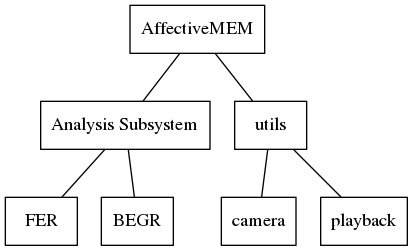
\includegraphics[width=.9\linewidth]{img/wbs1.png}
\caption{\label{fig:affheir}
Task in terms of complexity}
\end{figure}



The figure \ref{fig:affheir} shows an approximate overview of the entires system. The picture is not intended to give you an idea of how those subsystems will interact. It is there to show you what components we will be creating and working on in terms of the workbreakdown structure. In contrast, figure \ref{fig:affheir2} shows the actual work breakdown structure we planned for the only iteration in FYP 1.

\begin{figure}[htbp]
\centering
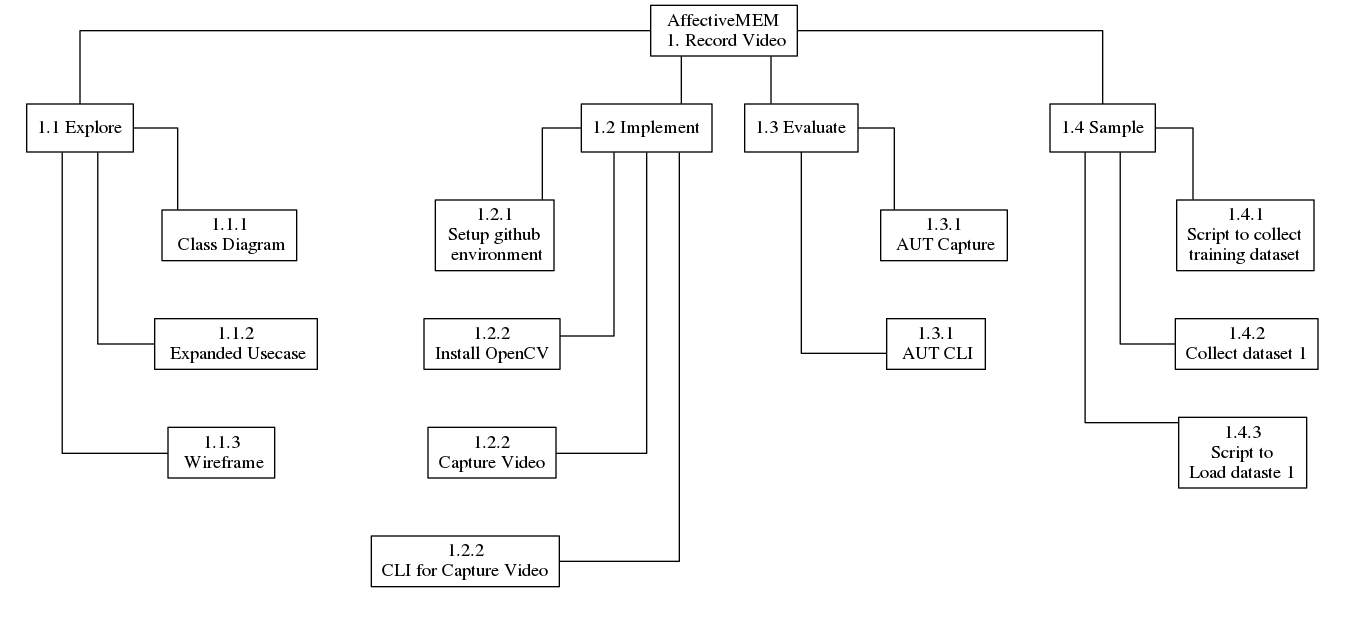
\includegraphics[width=.9\linewidth]{img/wbs2.png}
\caption{Work Breakdown Chart}
\end{figure}


\begin{table}[htbp]
\caption{\label{table:wbs_table}
Work breakdown tasks}
\centering
\begin{tabular}{|l|l|l|l|l|lp{3cm}|}
\hline
\textbf{Phase} & \textbf{Task} & \textbf{Start} & \textbf{Finish} & \textbf{Size}\\
\hline
1 & 1. Class Diagram & 12/03/19 & 16/03/19 & M\\
 & 2. Expanded Use-case & 12/03/19 & 16/03/19 & S\\
 & 3. Wireframe & 12/03/19 & 16/03/19 & S\\
\hline
2 & 1. Setup github &  &  & S\\
 & environment &  &  & \\
 & 2. Install OpenCV &  &  & S\\
 & 3. Capture Video &  &  & L\\
 & in a folder &  &  & \\
 & 4. CLI to Capture &  &  & M\\
 & Video &  &  & \\
\hline
3 & 1. AUT Capture &  &  & M\\
 & 2. AUT CLI &  &  & S\\
\hline
4 & 1. Script to collect &  &  & M\\
 & training dataset &  &  & \\
 & 2. Collect dataset 1 &  &  & L\\
 & 3. Script to load &  &  & M\\
 & dataset1 &  &  & \\
\hline
\end{tabular}
\end{table}



\chapter{Risk Management Plan}
\label{sec:org7bfb6ec}


\begin{table}[htbp]
\caption{\label{table:riskmgmt}
Risk Management Plan}
\centering
\begin{tabular}{|l|l|l|l|l|lp{3cm}|}
\hline
\textbf{\#} & \textbf{Description} & \textbf{Probability} & \textbf{Impact} & \textbf{Mitigation Strategy}\\
\hline
1 & Cannot collect dataset & 40\% & 4 & Use online reaction videos\\
 & to test movie evaluation &  &  & for shorter movie clips.\\
 & system. &  &  & \\
\hline
2 & Insufficent memory to train & 20\% & 4 & Ask the department for cloud\\
 & the model &  &  & computer access or more\\
 &  &  &  & physical computer resources\\
\hline
3 & Evaluation model is not & 5\% & 2 & Use another mean to take\\
 & performing as expected, &  &  & the measurements, use a\\
 & because features extracted &  &  & thermal camera or heartbeat\\
 & are not sufficent to &  &  & measuring instrument. If\\
 & represent properly &  &  & possible use new measurements\\
 &  &  &  & to create a baseline to\\
 &  &  &  & compare the evaluation model.\\
\hline
\end{tabular}
\end{table}

\chapter{Project timeline}
\label{sec:org71357b5}
You can find our baseline gantt chart for estimated project plan in Appendix A. We created the work breakdown structure during our project plan, and we grouped each task under a phase in our methodology. Then we estimated time for each task and prioritsed them, finally creating a project timeline in a gantt chart format. 

\begin{figure}[htbp]
\centering
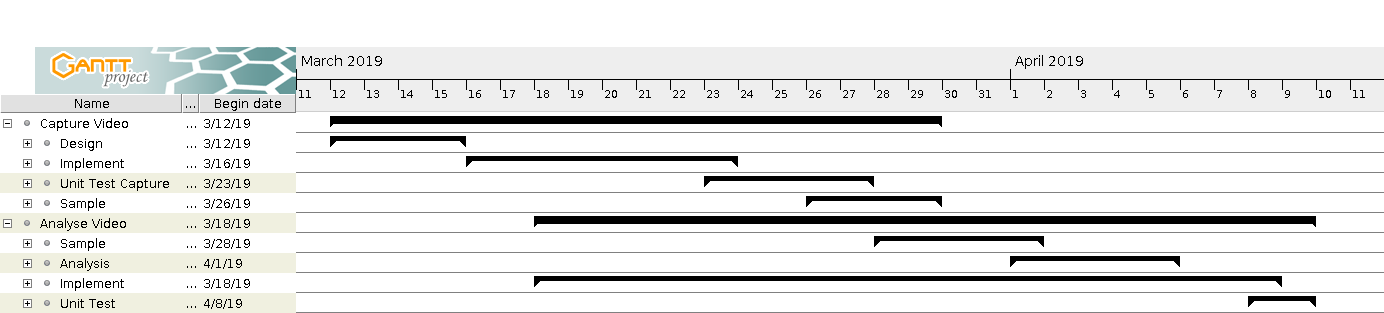
\includegraphics[width=7in]{./ext_img/gant1.png}
\caption{\label{fig:gantt1}
Overview of baseline gantt chart}
\end{figure}


\part{Requirement Analysis}
\label{sec:orgc1e0ccd}
\chapter{Introduction}
\label{sec:org19f8269}
Since the conception of the project plan, our initial goal for the first iteration was to create a system that is going to analyse the facial emotion and body posture emotion independently and construct a data representation such as a time-series from the analysis. We delegated the primary goal of our project, which is to use that data to train and create a model that can score movies for later iterations intentionally, so it will give us time to reconsider our methods and also create dataset in between the downtime.

Like any other software developement project, our approach was to first of all analyse the system and identify. Practically, most of the requirement analysis was done while we were creating the project plan, while we did not thoroughly document it in the proposal itself. This part of the document was later updated to reflect the change in number of use-cases in our iteration 1, after we realised that we are not able to fit the three initial use-cases we planned into the first iteration.

Along with the project's functional requirements and non-functional requirements, we will also try to give an overview of the requirements from the machine learning perspective. We will try to state the ML problem, and define the requirements and structure for the problem. It should be noted by now, our system will consist multiple ML algorithms interacting with each other and a portion of has to be designed by us. 

We also wanted to complete all the software design and engineering intensive tasks as early as possible so we can focus on the machine learning aspects of our project. Thus, a large portion of this iteration is writing the code for user interaction, and designing processes within the system that can perform independent of the type of user interface.

Initially, we like we planned we worked on the facial analysis, and posture analysis portion of the code seperately. Later on we refactored and integrated the code as seperate modules into a single codebase with the help of object-oriented programming.


\chapter{Requirement Summary}
\label{sec:orgfac6e78}
The first thing we did during our first meeting was infact to identify all the stakeholders and actors who interacted with the system. While we discussed the naming conventions of the actors involved during the later meetings, it was early on established that only one user directly interacts with the system and can be considered to be the primary user.

Our systems consists of mainly this one user controlling the application directly. Ideally this user is a system operator, hired by the production company with a knowledgeable background in IT and system administration. Throughout this document we refer to this user, simply as \emph{Admin}. We should note that the user \emph{Admin} is not really a recognized object within the system and thus does not have a login function. \emph{Admin} refers to whoever is operating the system.

\section{Actors and Stakeholders}
\label{sec:org4dfc943}
\subsection{Admin}
\label{sec:orged5502c}

An \emph{Admin} can use the system to record audiences watching a movie. Right now, in order to do that, the movie must exist within the computer system first. Admin is supposed to launch our application, and provide the details of the audience member and the movie, because the system does not yet store the metadata of the movies yet. The movie object is not considered as an object of the system in this iteration.

\begin{itemize}
\item Admin is able to Record a video of a \emph{Subject} watching a movie.
\item Admin is able to Analyse a video of a \emph{subject}
\begin{itemize}
\item Produce time-series.
\end{itemize}
\end{itemize}

\subsection{Subject}
\label{sec:org1d786ff}
Subject is not considered a primary actor in the system. The only interaction between the subject and the system occurs when the admin records the subject watching a movie in the first use-case. The admin initiates the use-case and subject passively sits infronts of the camera, until the movie is completed, whole while the admin actually have the control of the system such that they can terminate the recording process or wait until the movie is finished.

While the UML for iteration 1 might not directly hint that our system considers \emph{Subject} as a seperate entity for design purpose, it is going to be added as an Object in our future iteration. We did not include the \emph{Subject} as an object that is in the system, yet. 


\section{Object represented in the system}
\label{sec:org890aa69}
For this iteration, all use-cases are going to be involved with only two object. Object Sample represents a sample recording of an audience video, while the object movie represents a Movie that an audience is watching. It is important that these two logical objects are well defined within the system, as we might later need to categorize and display the statistics for future use cases.
\begin{figure}[htbp]
\centering
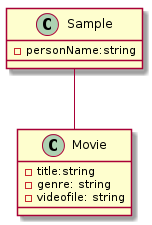
\includegraphics[width=2in]{./img/obj1.png}
\caption{\label{fig:gantt1}
Objects in the system}
\end{figure}


\chapter{Functional Requirements}
\label{sec:orgd2e22b6}
\section{Use-Case Diagrams}
\label{sec:org4f7250a}
While designing of the use-cases we only thought from a logical/business perspective and not included the "technical" usecases, as our methodology and approach does not heavily rely on UML. 



\begin{figure}[htbp]
\centering
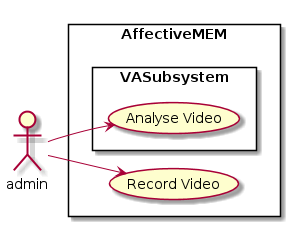
\includegraphics[width=3in]{./img/auc.png}
\caption{\label{fig:auc}
Iteration 1: Before integration}
\end{figure}


In figure \ref{fig:auc}, you can see that the Analyse Video is bound within a subsystem of Affective Movie Evaluator. The reason

While there is a weak implementation of other use cases, the two use-cases shown in the diagram \ref{fig:auc}, are the main goal of our current iteration until now.

\begin{figure}[htbp]
\centering
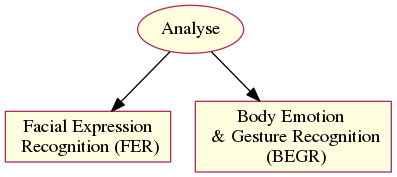
\includegraphics[width=5in]{./img/auc_exp.png}
\caption{\label{fig:auc}
Analyse uscase with subsystems}
\end{figure}


It would have been ideal for the sake of this documentation for Analyse use case to include two "technical" use-cases, "Analyse FER" and "Analyse BEGR", so that it is easier to credit the two team members, but it would not have been accurate. Ideally a use case should show an added value to a system, and seperating them does not really contribute the value to from either logical or design perspective. 

\section{High-Level Use Cases}
\label{sec:org78c43e4}

\begin{table}[htbp]
\caption{\label{table:auc1}
Analysis usecases}
\centering
\begin{tabular}{|l|l|lp{3cm}|}
\hline
\textbf{Use Case 1} & Record Video  \footnotemark\\
\hline
Goal in Context & To record an audience member's video and store it.\\
\hline
Primary Actors & - Admin\\
Secondary Actor & - Audience\\
\hline
Description & Use camera to record and store video session of an audience\\
 & watching a movie screening.\\
\hline
\hline
\textbf{Use Case 2} & Analyse Video \footnotemark\\
\hline
Goal in Context & To extract an audience's facial and body pose data from a\\
 & video file and store it as readable data.\\
\hline
Primary Actors & - Admin\\
Secondary Actor & - Audience\\
\hline
Description & Use camera to record and store video session of an audience\\
 & watching a movie screening.\\
\hline
\end{tabular}
\end{table}\footnotetext[1]{\label{orgc68c435}Use case was designed by faith and implemented by Ibrahim.}\footnotetext[2]{\label{orgabef40d}FER portion of use-case was created by Faith and BEGR was created by Ibrahim.}


\chapter{Non-Functional Requirements}
\label{sec:orgb0a2e85}
\section{Technical Requirements}
\label{sec:orgee7a128}
\subsection{Prototype 1 - BIT304}
\label{sec:org9ce3f7c}
We recommend to use a moderately powerful desktop computer to run the application. For video capture, it currently uses a webcam, though the application is currently compatible with any other type of live video capture stream. Ideally, a dual monitor system must be used one facing the audience and one facing the \emph{Admin}, who will be interacting with the control panel. The system was actually tested on a laptop computer and we assume that it is also possible to setup and run this application on most standard laptops without any issue. 

Almost all of our application is written using Python 3. We used the Anaconda distribution of python and it's environment and package management system because it reduced the compatibility issues associated with installing packages such as tensorflow across different systems. 

\begin{table}[htbp]
\caption{\label{table:minreq1}
Minimum Software Requirements}
\centering
\begin{tabular}{|l|l|lp{3cm}|}
Software\\
\hline
Windows 7/8\\
\\
\end{tabular}
\end{table}

\begin{enumerate}
\item Recommended Setup
\label{sec:orgfadf8d5}
\begin{itemize}
\item Linux based system, preferrably Debian variant
\item System Utilites
\begin{itemize}
\item git
\item conda
\end{itemize}
\item Intel based processor preferrably greater than 5th Generation i5
\item 8GB RAM
\end{itemize}
\end{enumerate}

\section{Usability Requirements}
\label{sec:org6bac26b}

Our standard user documentation is written as a README file in markdown format. Since the project is currently available in GitHub, the documentation is the first thing the user can see of our project. The purpose of the user documentation is to describe the whole project briefly, and guide the user to install and setup the application.

The user is able to interact with the application through commandline and GUI.

\section{Reliability Requirements}
\label{sec:org5671332}
In our current iteration, all the files are stored in the filesystem within the project file. Our version control system (git) does not track the data files and models, since they are considered large and we do not think it will be effective to use VCS to track data files. Therefore, datasets and results must be shared and versioned manually, we will have to back it up separately and share it on internet with email and file sharing services.

One of the scripts we wrote that will run when a new user is going to setup the system, will actually download the pre-trained models used by subsystems from the internet. This seems to be a standard practice as even larger projects such as OpenPose often does not store their models in the github repository. 

\section{Security Requirements}
\label{sec:orgc38cd95}
By design, our system does not have an authentication system nor it is considered required. We consider that if deployed, most production studios have their own security systems to control access.

The only time the application uses network currently is to access the internet and download the required models and software.

One concern a production studio may have is regarding the security of test audience data that is stored. Depending on the contract they have with their own test audience, the test audience may be concerned with their privacy if the data is leaked or shared without their permission for other projects.


\subsection{FYP2}
\label{sec:org9623326}
We plan to implement the cloud analysis use-case for iteration 3.


\part{Iterations}
\label{sec:orgec5cacb}
\chapter{Iteration Plans}
\label{sec:org929cd1a}
Early on we planned two iteration for FYP 1, but as mentioned in the requirement analysis we had to change that because of time constraint and risks of not completing the objectives of our FYP 1. 

As shown in our project timeline, we combined SEMMA phases with SDLC phases in our project timeline. The SEMMA phase are not analogous to an SDLC phase, and we've learned that there may exist no standard for such analogy. For example most software engineers and feature engineers tend to write code during the Sample phase while ML engineers may work on something else. For later iterations, we are going to follow the SEMMA phases more rigidly as we will be working more on the machine learning aspects of the project.


\section{Current Iteration}
\label{sec:org32b2256}
We only have one Iteration for this part of our final year project. Initially the work was divided between the two part. Use case one was primarily developed by Ibrahim and designed by Faith. Use-case two's main two sub-components were developed and tested independently and later on we re-integrated our work into a single codebase.

\begin{table}[htbp]
\caption{\label{table:iterplan}
Iteration Plan}
\centering
\begin{tabular}{|l|l|l|l|l|lp{3cm}|}
\hline
\textbf{FYP} & \textbf{Iteration} & \textbf{Use Cases} & \textbf{Proposed Start Date} & \textbf{Proposed End Date}\\
\hline
1 & 1 & 1,2 & 11/03/19 & 09/04/19\\
 &  &  &  & \\
\hline
2 & 2,3 & 2,3,4 &  & \\
\hline
\end{tabular}
\end{table}


\section{Future Iterations}
\label{sec:org99777f2}

\begin{table}[htbp]
\caption{\label{table:fuiterplan}
Future Iterations}
\centering
\begin{tabular}{|l|l|l|l|lp{3cm}|}
\hline
\textbf{Iteration} & \textbf{Use Cases} \footnotemark\\
\hline
2 & 3, 4\\
3 & 4, 5\\
\hline
\end{tabular}
\end{table}\footnotetext[3]{\label{org58ff1e8}Future use cases are described under the conclusion chapter.}


\chapter{Iteration 1}
\label{sec:org06e6645}
\section{Introduction}
\label{sec:org0a2d6b6}
Like we mentioned before this iteration implements only two use-cases, but it does not mean the amount of tasks we have is smaller than iteration 2, which we have planned that involves more use-cases. Our plan for this iteration was changed throughout the developement, project. Initially we had 2 iterations and considered adding more use-cases that manages movies and samples within the system. However once we finished our work breakdown and started to sort out our tasks, we figured out it will be a risk considering all the tasks we have and we might not be able to complete our goals within timespan. 

So iteration 1 was expanded to cover most of this semester and we focused on two use-cases from the user-perspective. From the system perspective, we started working on the two main analysis subsystems once our on use-case two commenced. 

\section{Purpose}
\label{sec:org49c0758}
The purpose of this iteration is mainly to make sure our application can record a video and extract the primary data, required for machine learning from the video. This means the two analysis subsystems must be designed tested, and they should be integrated into the system.

By the end of this iteration the system should be able to do the following:
\begin{enumerate}
\item \textbf{Capture Video}: The admin should be able to record video by using the command line interface and graphical user interface, to create a video file.
\item \textbf{Analyse Video}: The admin must be able to create time-series data from an existing recording of a subject.
\end{enumerate}


\section{Context}
\label{sec:org585884f}
On a grand scale, by the end of this iteration we will have a codebase and an fixed project structure. It should be easier to navigate and design for our future iterations, since we will be more familiar with how we are going to work and what exactly needs to be documented. Most importantly, the review of the first iteration is actually going to help us estimate and prioritize the tasks for future iterations because it is going to show how much we overestimate or under-estimate the size of a task.

\section{Schedule of Iteration Workflow}
\label{sec:org7f5d974}
\begin{longtable}{|l|l|l|l|l|l|l|lp{3cm}|}
\caption{\label{table:iterwork}
Schedule of Iterations Workflow}
\\
\hline
\textbf{Workflow} & \textbf{Start} & \textbf{End} & \textbf{Duration}\\
\hline
\endfirsthead
\multicolumn{4}{l}{Continued from previous page} \\
\hline

\textbf{Workflow} & \textbf{Start} & \textbf{End} & \textbf{Duration} \\

\hline
\endhead
\hline\multicolumn{4}{r}{Continued on next page} \\
\endfoot
\endlastfoot
\hline
\textbf{1.Capture Video} & 11/03/19 & 30/03/19 & 19 days\\
Design & 11/03/19 & 16/03/19 & \\
Implement & 16/03/19 & 24/03/19 & \\
Evaluate & 22/03/19 & 28/03/19 & \\
Sample & 26/03/19 & 30/03/19 & \\
\hline
\textbf{2. Analyse Video} & 18/03/19 & 09/04/19 & 22 days\\
Sample & 29/03/19 & 02/04/19 & \\
Explore/Design & 01/04/19 & 06/04/19 & \\
Implement & 18/03/19 & 09/04/19 & \\
Modify & 08/04/19 & 09/04/19 & \\
Test & 08/04/19 & 09/04/19 & \\
\hline
\end{longtable}


\section{Iteration Schedule Breakdown}
\label{sec:org83fa812}

\begin{longtable}{|l|l|l|l|l|l|l|lp{3cm}|}
\caption{\label{table:itersched}
Schedule of Tasks}
\\
\hline
\textbf{Use case} & \textbf{Task Name} & \textbf{Start} & \textbf{Finish} & \textbf{Est Time}\\
\hline
\endfirsthead
\multicolumn{5}{l}{Continued from previous page} \\
\hline

\textbf{Use case} & \textbf{Task Name} & \textbf{Start} & \textbf{Finish} & \textbf{Est Time} \\

\hline
\endhead
\hline\multicolumn{5}{r}{Continued on next page} \\
\endfoot
\endlastfoot
\hline
 & \textbf{1.1 Design (Explore)} & 11/03/2019 & 16/03/2019 & 5\\
1 & 1.1.1 Class Diagram &  &  & \\
 & 1.1.2 Expanded Use-Case &  &  & \\
 & 1.1.3 Wireframes &  &  & \\
\hline
1 & \textbf{1.2 Implement} & 16/03/19 & 24/03/19 & 8\\
 & 1.2.1 Setup github environment &  &  & \\
 & 1.2.2 Install OpenCV &  &  & \\
 & 1.2.3 Capture video in a folder &  &  & \\
 & 1.2.4 CLI to capture video &  &  & \\
\hline
1 & \textbf{1.3 Evaluate} & 22/03/19 & 28/03/19 & 6\\
 & 1.3.1 AUT capture &  &  & \\
 & 1.3.2 AUT CLI &  &  & \\
\hline
1 & \textbf{1.4 Sample} & 26/03/19 & 30/03/19 & 4\\
 & 1.4.1 Script to collect training dataset &  &  & \\
 & 1.4.2 Collect Test Dataset 1 &  &  & \\
 & 1.4.3 Write script to load test dataset &  &  & \\
\hline
2 & \textbf{2.1 Sample} & 29/03/19 & 02/04/19 & 4\\
 & 2.1.1 Collect Test Dataset 2 &  &  & \\
 & 2.1.1 Download FER dataset &  &  & \\
 & 2.1.2 Script to load FER dataset &  &  & \\
\hline
2 & \textbf{2.2 Explore/Design} & 01/04/19 & 06/04/19 & 5\\
 & 2.2.1 Split and label Test Dataset 2 &  &  & \\
 & 2.2.2 Pipeline Diagram &  &  & \\
 & 2.2.3 Interaction Diagram (SSD) &  &  & \\
 & 2.2.4 Design Class Diagram &  &  & \\
 & 2.2.5 Wireframe &  &  & \\
\hline
2 & \textbf{Implement} & 18/03/19 & 09/04/19 & 22\\
 & 2.3.1 Setup FER library &  &  & \\
 & 2.3.2 Setup OpenPose Library &  &  & \\
 & 2.3.3 Generate FER time series &  &  & \\
 & 2.3.4 Generate Pose time series &  &  & \\
 & 2.3.5 Integrate FER analysis to UI &  &  & \\
 & 2.3.6 Integrate BEGR analysis to UI &  &  & \\
 & 2.3.7 Analyse Video CLI &  &  & \\
\hline
2 & \textbf{2.4 Modify} & 07/04/19 & 09/04/19 & 2\\
 & 2.4.1 Define combined time-series file format &  &  & \\
 & 2.4.2 Code to Visualise Time Series &  &  & \\
 & 2.4.3 Refactor code &  &  & \\
\hline
2 & \textbf{2.5 Evaluate} & 07/04/19 & 09/04/19 & 2\\
 & 2.5.1 Write automated unit test &  &  & \\
 & 2.5.2 FER Accuracy test &  &  & \\
 & 2.5.3 Pose accuracy test &  &  & \\
\hline
\end{longtable}


\section{Resource Summary}
\label{sec:org911b444}
Resources used for this project
\begin{longtable}{|l|l|l|l|l|l|l|lp{3cm}|}
\caption{\label{table: hard_ressumm}
Hardware Resources used for iteration}
\\
\hline
\textbf{No} & \textbf{Hardware} & \textbf{Usage} & \textbf{Qty}\\
\hline
\endfirsthead
\multicolumn{4}{l}{Continued from previous page} \\
\hline

\textbf{No} & \textbf{Hardware} & \textbf{Usage} & \textbf{Qty} \\

\hline
\endhead
\hline\multicolumn{4}{r}{Continued on next page} \\
\endfoot
\endlastfoot
\hline
1 & Laptops with & Testing & 2\\
 & webcams & and Developement & \\
\hline
2 & HD Webcam & Capture sample & 1\\
 &  & and testing & \\
\hline
3 & Microsoft Azure & To speed up analysis & 1\\
 & Cloud VM & for testing purpose & \\
\hline
\end{longtable}


Software Resources used for this project
\begin{longtable}{|l|l|l|l|l|l|l|lp{3cm}|}
\caption{\label{table: soft_ressumm}
Software Resources used for iteration}
\\
\hline
\textbf{No} & \textbf{Software} & \textbf{Usage} & \textbf{Qty}\\
\hline
\endfirsthead
\multicolumn{4}{l}{Continued from previous page} \\
\hline

\textbf{No} & \textbf{Software} & \textbf{Usage} & \textbf{Qty} \\

\hline
\endhead
\hline\multicolumn{4}{r}{Continued on next page} \\
\endfoot
\endlastfoot
\hline
1 & Python 3 & Programming language & 1\\
 & (conda distribution) & and runtime environment & \\
\hline
2 & Tensorflow & A lower level machine & 1\\
 &  & learning API for python which & \\
 &  & interacts with hardware, & \\
 &  & used to train, load and & \\
 &  & predict ML/DNN models. & \\
\hline
3 & Keras & A higher level python library which can & 1\\
 &  & be used as an abstraction over & \\
 &  & tensorflow, or other lower level API. & \\
 &  & Like tensorflow optimized for deep & \\
 &  & deep learning and general ML tasks, but & \\
 &  & more simple to use. & \\
\hline
4 & Click & Python libary used to create the & 1\\
 &  & command line interface & \\
\hline
5 & wxPython & Python implementation of the popular & 1\\
 &  & wx widgets toolkit. Used to create our & \\
 &  & GUI & \\
\hline
6 & pytube & Enables python script to interact with youtube. & 1\\
 &  & We use this in data collection scrips and & \\
 &  & also by scripts to download the test case movies. & \\
\hline
7 & OpenCV python & Python API for OpenCV library. OpenCV & \\
 &  & is the standard toolkit used to manipulate & \\
 &  & images and computer vision tasks. We use it for & 1\\
 &  & variety of purpose including reading from & \\
 &  & webcam and performing image manipulations. & \\
\hline
\end{longtable}

\section{Evaluation Criterea}
\label{sec:orgd99dd83}

The criteria for evaluation of the whole system is divided into three parts. We intend to test the software 
\begin{enumerate}
\item FER Evaluation
\item BEGR Evaluation
\end{enumerate}

The approach to test the \emph{Software 1.0} parts and the \emph{Software 2.0} (machine learning) parts of the system are very different.
The software engineering aspects and machine learning parts of the code must be tested using very serpe

In this iteration we do not evaluate the speed and accuracy performance of the entire pipeline, from the beginning, something we intend to do in all the future iterations.


\section{Analysis and Design Artefacts}
\label{sec:org808e222}
\subsection{Pipeline diagrams}
\label{sec:orgcd692a0}

\begin{center}
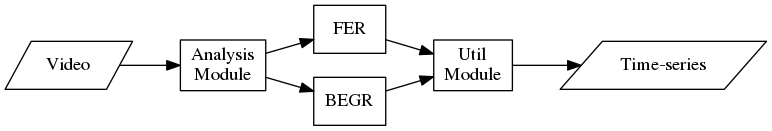
\includegraphics[width=.9\linewidth]{img/pipeline.png}
\end{center}


Even though it is possible to run \emph{FER} and \emph{BEGR} simultaneous and in parallel by design, during the implementation phase we realised our development systems are not capable of  running the subsystems in parallel without running out of memory. Therefore, we decided that the video will pass through the analysis pipeline twice to exctract the time-series data.


\begin{center}
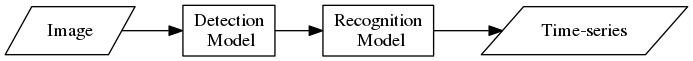
\includegraphics[width=.9\linewidth]{img/ferpipeline.png}
\end{center}


\begin{center}
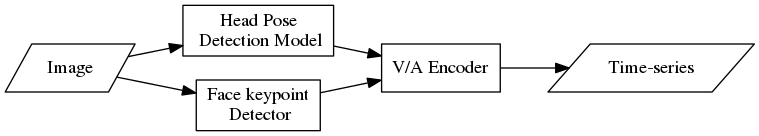
\includegraphics[width=.9\linewidth]{img/begrpipeline.png}
\end{center}

The valence arousal encoder is currently not built, instead we use a hard coded module as a replacement. Currently all the V/A encoder returns is a 1 dimensional value that we call 'interest'. If the subject is facing the camera the algorithm returns a higher value, otherwise we return a lower value.


\subsection{Class Diagrams}
\label{sec:orgd22620c}
The design class diagram shown here has been updated to represent the actual implementation faithfully. The actual deliverables we made before the change can be found in the design doc folder of along with the source code. By glancing at the class diagram we can say that the structure is not consistent,  since we followed the agile principle of "document what you need", the requirements were kept brief before we implemented each work item.

\begin{center}
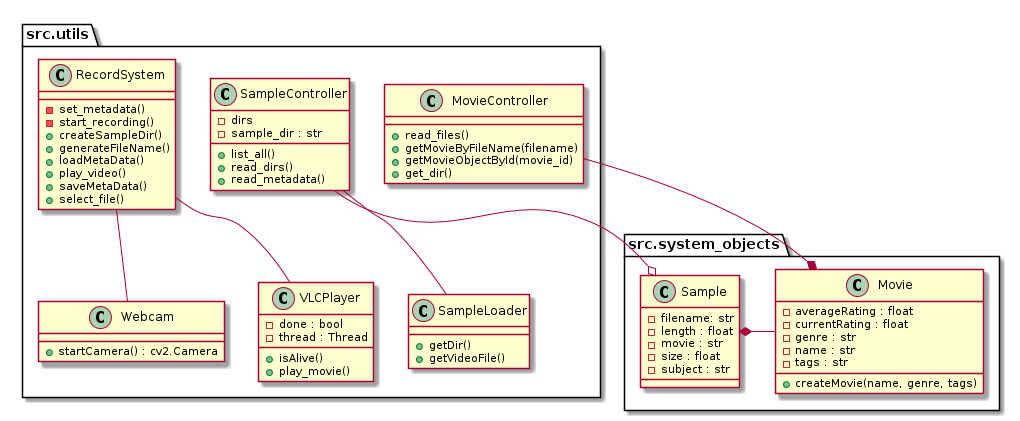
\includegraphics[width=.9\linewidth]{img/class1.png}
\end{center}

The classes RecordSystem, SampleController and MovieController are respectively used by the User interface code for the use case. We do not have a presentation layer abstraction between the actual user interface code and the \emph{Controller} classes.

One design principle we tried to follow loosely is the Single-Responsible principle, as you can see from the diagram. A class should have one responsibility, but we did not adher strictly to it.

Webcam module helps setting up the camera.


\begin{center}
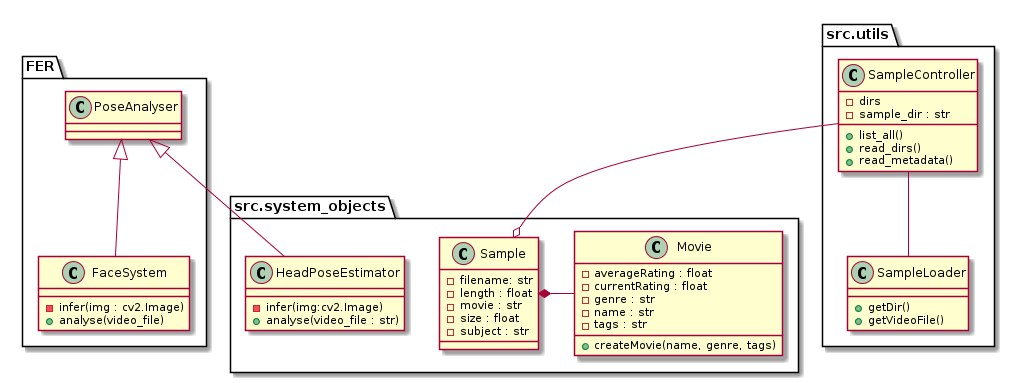
\includegraphics[width=.9\linewidth]{img/class2.png}
\end{center}

Note since the current BEGR subsystem's full body pose recognizer is too slow, we replaced it with another model only measuring head pose and renamed the package \emph{begr} as \emph{head\_pose}. Package \emph{head\_pose} is just a placeholder for \emph{begr} until we find a better replacement. 

Also, the fact that BEGR code is not in a seperate package and FER code is in a separate package, is because of a miscommunication and oversight between the two programmers who worked on this during the developement and we decided not to refactor the mistake until, next iteration due to lack of time. BEGR should be refactored into it's own package by in the future.

\chapter{Iteration I: Implementation and Testing}
\label{sec:org552b49b}

Our manual tests corresponds to the use-cases, for demonstration purpose we isolate the components associated with the use-case. We do this manual process only for the sake of documentation, while most other smaller systems are tested with the help of automated pythons automated unit testing framework.

\section{Implementation}
\label{sec:org3c6536b}
Our application is mostly written in python with the exception of few OS specific shell scripts used to setup and configure. For developement we used conda distribution of python, along with its package and environment manager. The main reason we chose conda was it's ease of use, when installing certain packages such as tensorflow for various platforms compared to pythons default package manager.

\begin{verbatim}
~/affective_movie_evaluator/$ conda create --name affmem_env \
						  pip tensorflow python=3.5
~/affective_movie_evaluator/$ conda activate affmem_env
~/affective_movie_evaluator/$ conda activate 
(affmem_env) ~/affective_movie_evaluator/$ 
\end{verbatim}

The shell command snippet above shows an example scenario of creating a conda environment and activating the environment for the project. Right now we recommend all \emph{Admins} to work using conda environment to avoid common multiple dependency version issues users face when they use the global python environment.


All of the data was stored directly on disk drive, and the system identifies the objects with the help of metadata written in JSON format. Since we are not expecting search functions, that will traverse through the disk drive and most machine learning algorithms either loads datasets in batches or in entirety we do not think a database is necessary. A search with the current system will perform linearly \(O(n)\) and an insertion will cost constant time.

\begin{figure}[htbp]
\centering
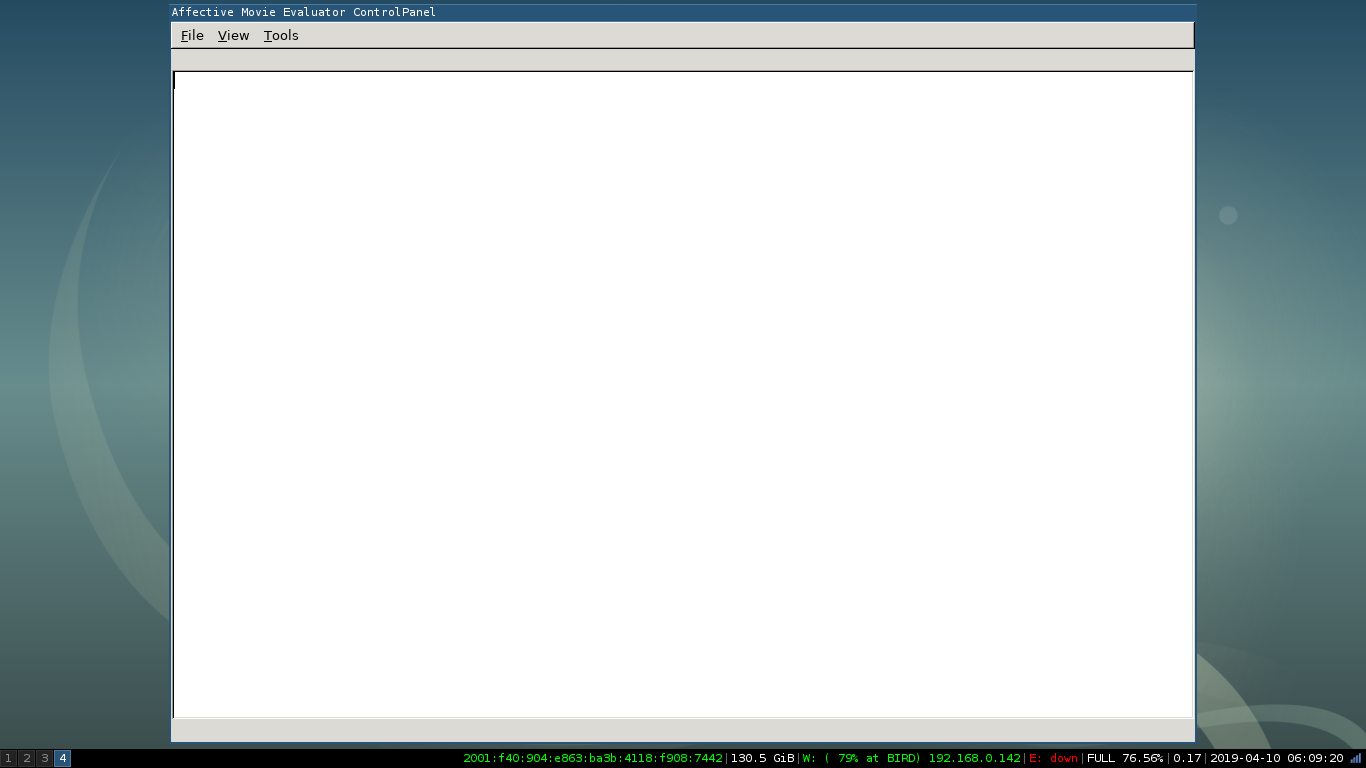
\includegraphics[width=5in]{./ext_img/sc1.png}
\caption{\label{fig:sc1}
The GUI Application}
\end{figure}

Figure \ref{fig:sc1} shows the initial screen the admin will see once they start the application. The empty text area shown in the screenshot is going to display error error messages for the admin, and was also used as the console log by us while were developing the application.

\begin{figure}[htbp]
\centering
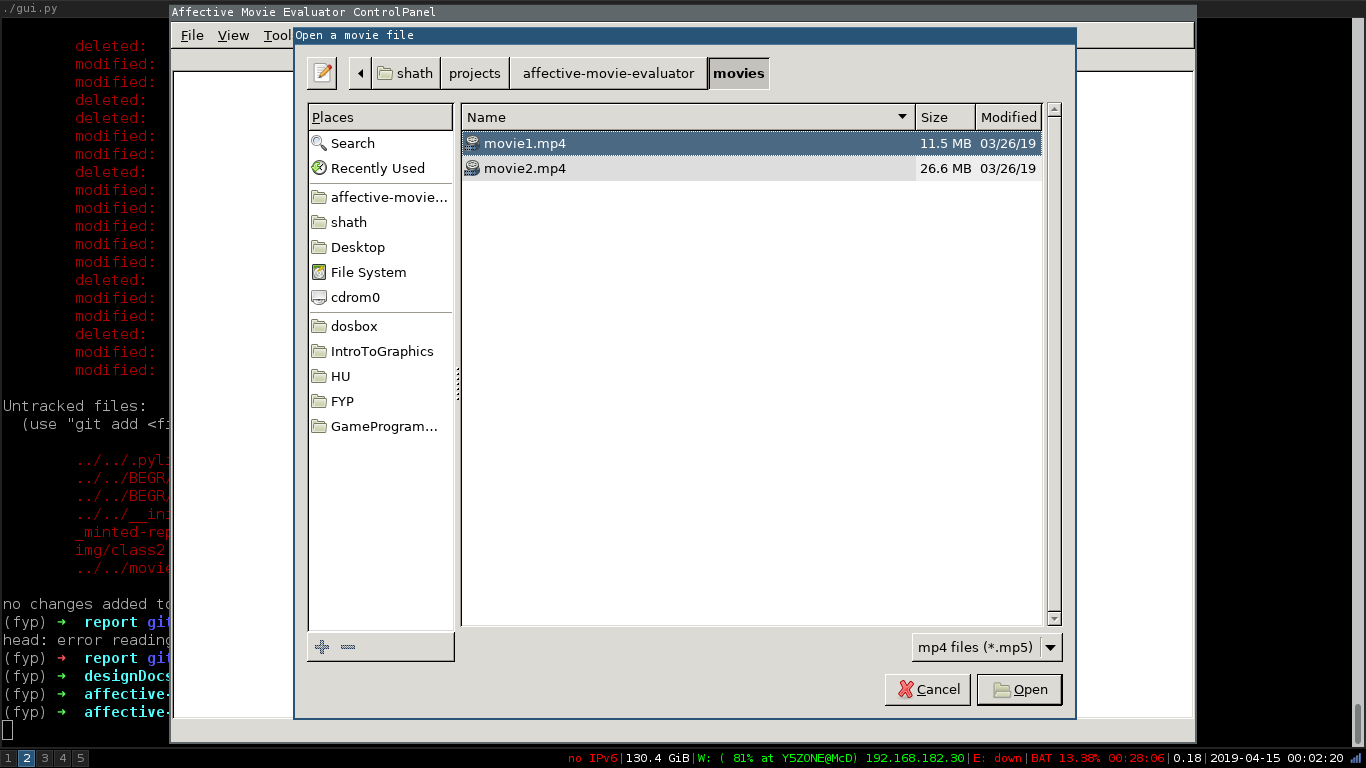
\includegraphics[width=5in]{./ext_img/sc1.1.png}
\caption{\label{fig:sc12}
Record Sample: 1. Select the movie file}
\end{figure}

If the \emph{Admin} wants to record a new sample, they will have to select a movie stored from the disk drives. The movie files are stored in a the 'movies' directory as shown in Figure \ref{fig:sc12}, along with the metadata file which describes each movie.

Our overall strategy for implementation can be describe as a test driven bottom up approach. For modules that uses machine learning we have a different approach, instead of writing tests for accuracy or simple integration we write a procedural test file, then convert into Object Oriented code which is compatible with our Analyse interface.


\begin{figure}[htbp]
\centering
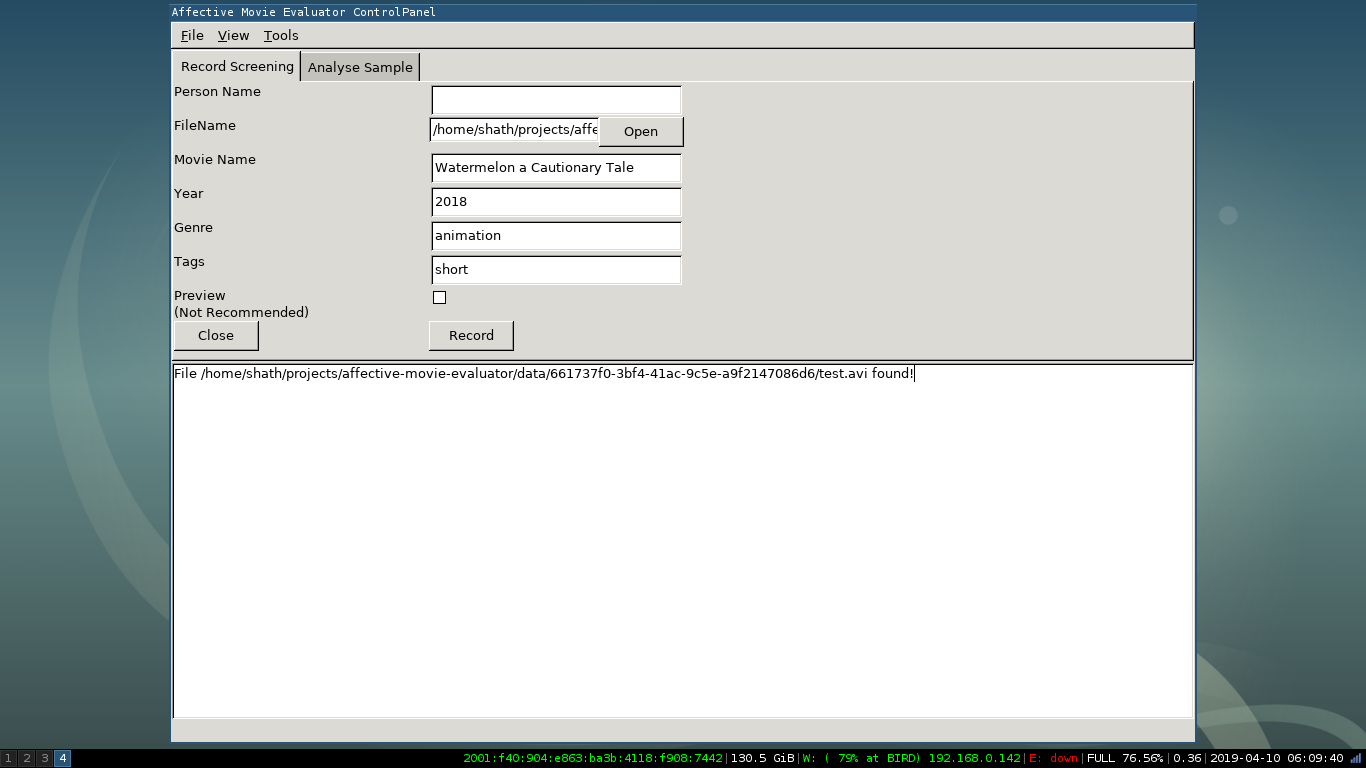
\includegraphics[width=5in]{./ext_img/sc2.png}
\caption{\label{fig:sc2}
Record Sample: 2. Fill in the blanks}
\end{figure}



\begin{figure}[htbp]
\centering
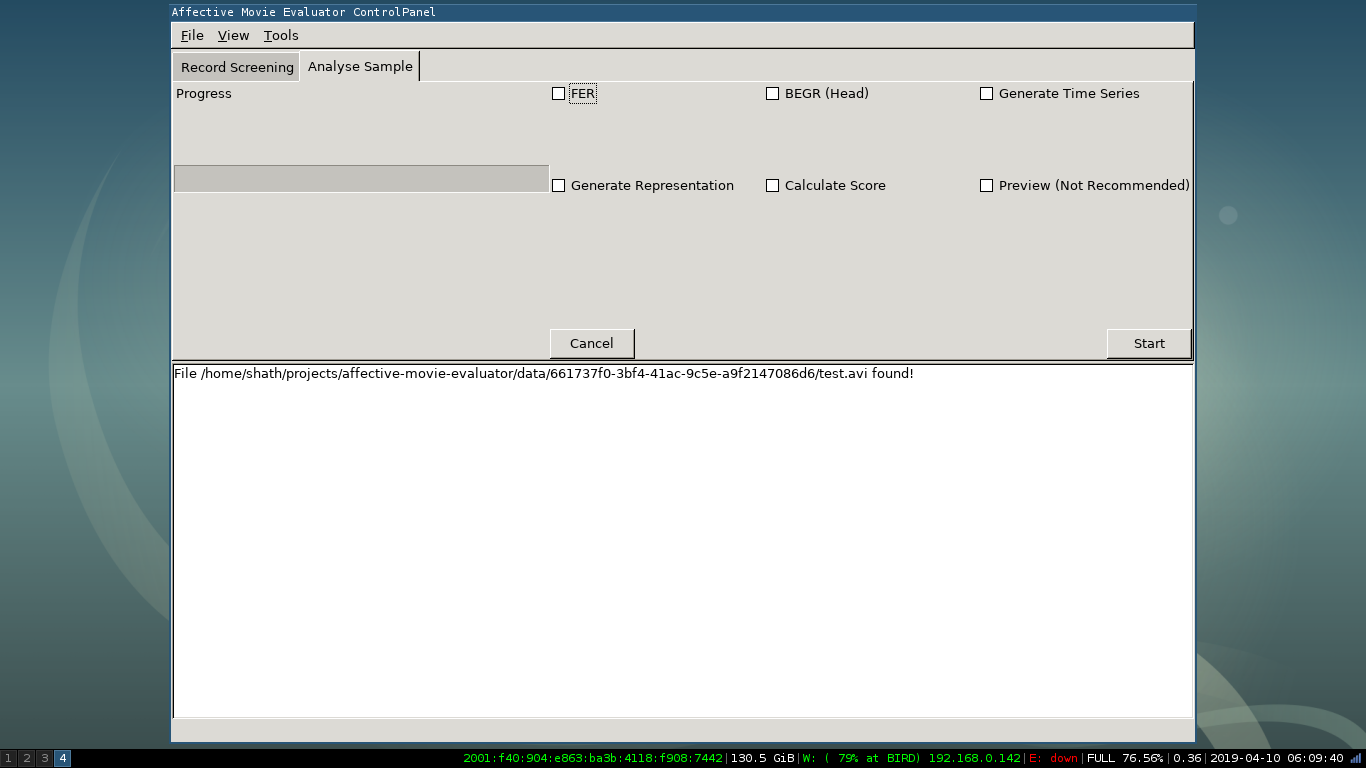
\includegraphics[width=5in]{./ext_img/sc3.png}
\caption{\label{fig:sc3}
Analyse Screen}
\end{figure}

\section{User Manual}
\label{sec:orgfab3090}
The user manual is supposed to be at the project directory folder, in markdown format. We do intent to write a more detailed user documentation on the final iteration, on how to operate and trouble shoot. The user documentation right now consists of how to setup and install, then the only two use cases. The system does have extra features that need to be documented so that the user can effectively operate the system.

In order to use the system the user must, setup python and installed required libraries listed in requirements.txt then run the scripts to download and install the models. Once the models are installed, the user can run the "./gui.py" to open the user interface. A brief overview of how it is used is described in the implementation section.

\section{Testing}
\label{sec:orgfdff9e0}


\begin{table}[htbp]
\caption{\label{table:strattable}
Table of Strategy}
\centering
\begin{tabular}{|l|l|l|l|l|lp{3cm}|}
\hline
\textbf{No.} & \textbf{Strategy}\\
\hline
1 & Create the smallest possible class\\
\hline
2 & Write the unit test for the class    and improve the class until it\\
 & passes all the basic test conditions\\
\hline
3 & Write the user interface code\\
\hline
\end{tabular}
\end{table}


\begin{table}[htbp]
\caption{\label{table:mstrattable}
Table of Strategy for Models}
\centering
\begin{tabular}{|l|l|l|l|l|lp{3cm}|}
\hline
\textbf{No.} & \textbf{Strategy}\\
\hline
1 & Write driver code for used for testing purpose\\
\hline
2 & Write the class which can import the model and\\
 & perform predictions\\
\hline
3 & Keep on improving the class until the\\
 & realtime tests pass\\
\hline
\end{tabular}
\end{table}

We did not use the main dataset and movie diretory for testing purpose, but instead created mock data for that purpose. For example, in order to test the SampleLoader which loads the Sample for other module given the parameter, we actually created a test directory without actual samples but metadata files. 

\begin{table}[htbp]
\caption{\label{table:testtable}
Test Plan}
\centering
\begin{tabular}{|l|l|l|l|l|lp{3cm}|}
\hline
\textbf{Type of testing} & \textbf{Approach} & \textbf{Subject}\\
\hline
 &  & \\
Automated Unit Testing & White & Unit: RecordSystem\\
Integration Testing & Black Box & Usecase 1, Usecase 2\\
\hline
\end{tabular}
\end{table}


\begin{table}[htbp]
\caption{\label{table:testt}
Test Plan}
\centering
\begin{tabular}{|l|l|l|l|l|lp{3cm}|}
\hline
\textbf{Type of testing} & \textbf{Approach} & \textbf{Use Case} & \textbf{Task}\\
\hline
Automated Unit Testing & White & 1. Record Video & \\
 &  &  & \\
\end{tabular}
\end{table}


All automated unit tests are prefixed with the letter A to distinguish it from manual tests, which are prefixed with the letter M. Manual unit testing requires user to run and observe the results for each test case, and tests may require user input unlike automated unit tests.

\part{Conclusion}
\label{sec:org7215711}
\chapter{Current Status}
\label{sec:orgbe190d9}
   So far we have been able to complete the most vital objectives. One of the failure of our FYP is that we prioritzed system development work items such as GUI developement over 
data collection and machine learning tasks. This is because we wanted to demonstrate the application as soon as possible.  
  Throughout the developement we were able to resolve most of the issues we faced with compromises which affects changes in the project. For example we prioritised speed, by often choosing less accurate model over models that can run in considerable time. This means often the models extract less features than we originally intended, and so far we cannot estimate how much of a difference that would make on our entire overall system.

So far, there are no clear results about how successful the project is going to be in terms of accuracy. Faith is planning to focus on improving the FER subsystem, and we might be able to detect and improve problems with the machine learning models in the pipeline once we the system is able to run the accuracy tests. Ibrahim will focus on building the BEGR and representation model, while both team members will contribute in other system developement work items.

We also plan to possibly experiment integrating our own deep learning model into the pipeline, possibly to build representation for the time-series. Currently, our strategy for representation algorithm is to visualize and cluster the time series representation using a unsupervised ML algorithm before we sent for regression/classification.

\part{Appendix A - Gantt Charts}
\label{sec:org13bdf6f}

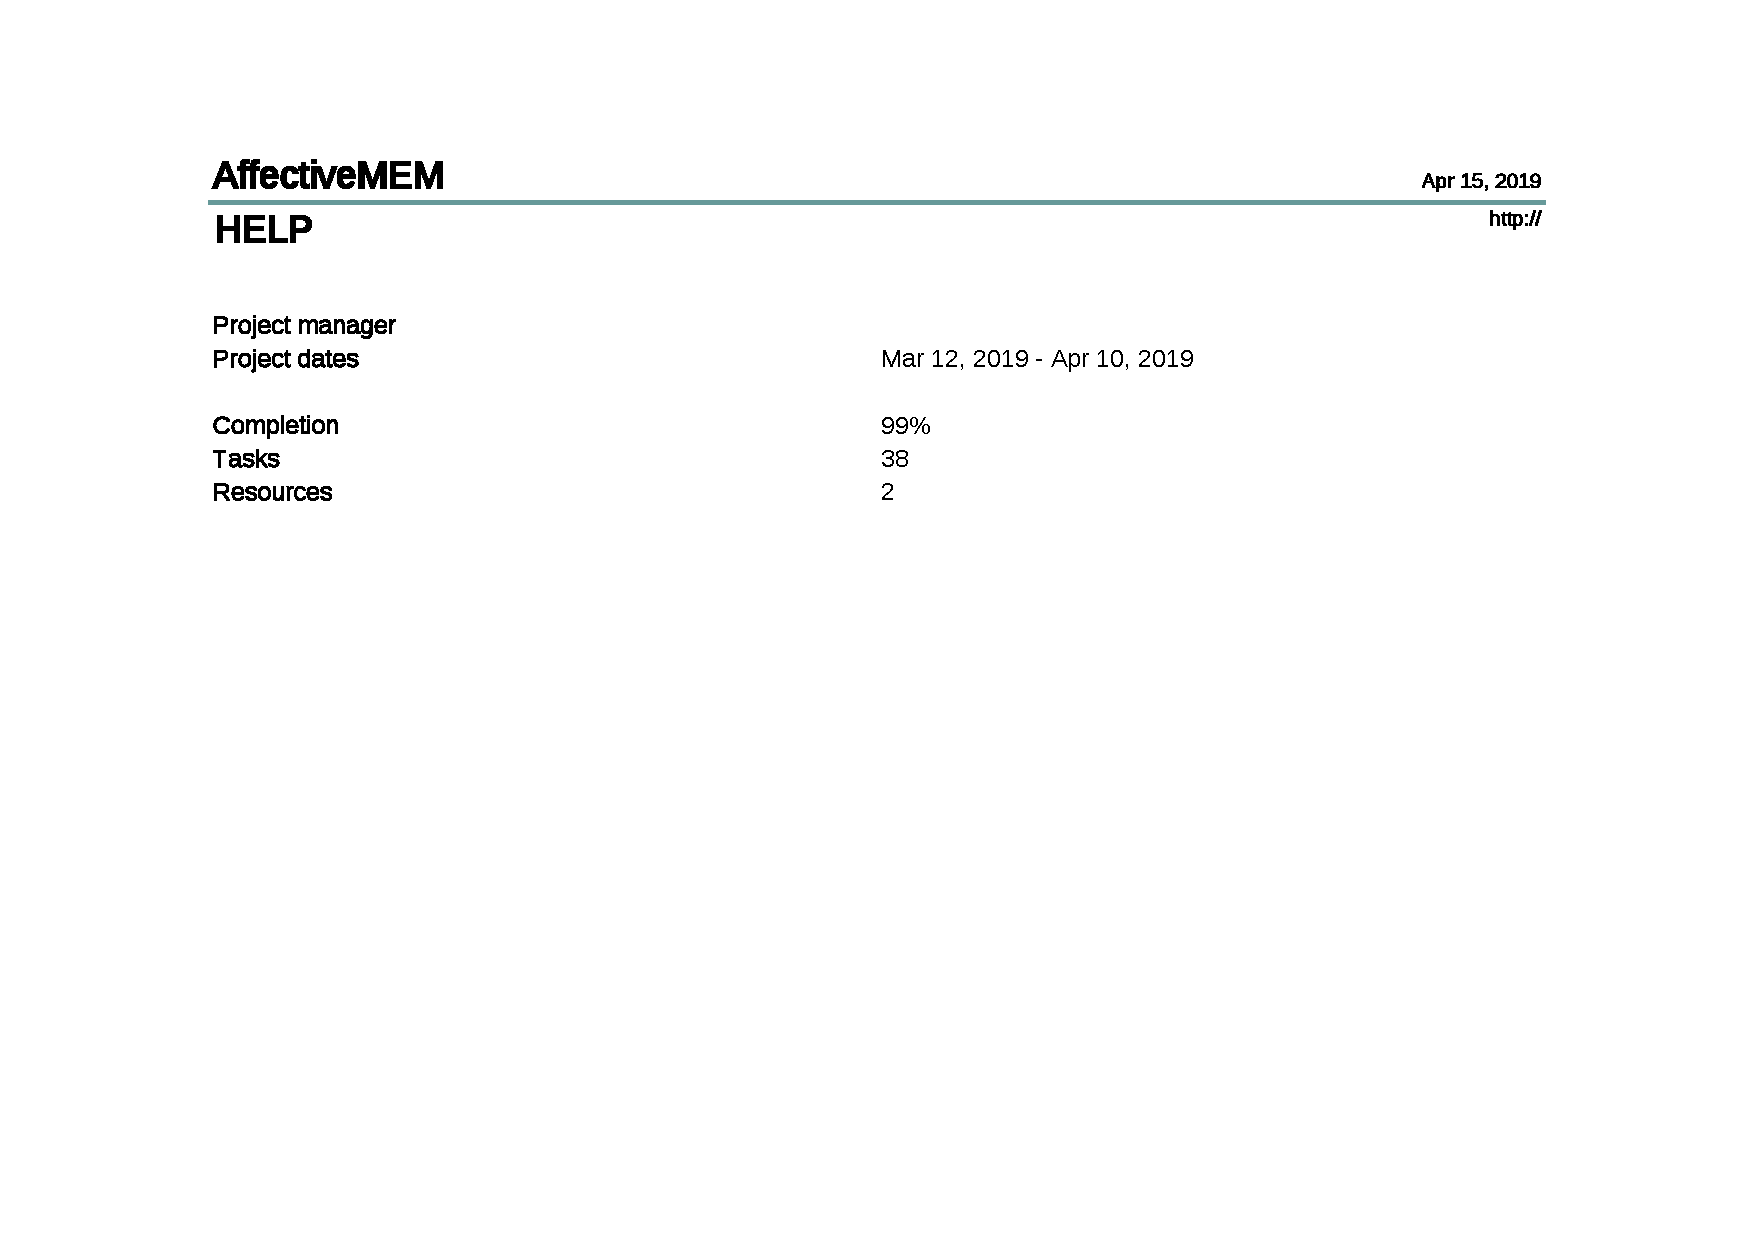
\includepdf[pages=-,pagecommand={},width=\textwidth]{gantt.pdf}

\part{Appendix B - Monthly Progress Reports}
\label{sec:org62e8931}


\part{Appendix C - Meeting Reports}
\label{sec:org7e54b73}


\part{Appendix D - Minutes}
\label{sec:org5494ce9}


\part{Appendix E - Evaluation Report}
\label{sec:org166ae8d}


\includepdf[pages=-]{ibrahim.pdf}


\includepdf[pages=-]{faith.pdf}

\part{Bibliography}
\label{sec:org2f8c352}
\printglossaries

\bibliographystyle{apacite}
\bibliography{ref}
\end{document}
